%%%%%%%%%%%%%%%%%%%%%%%%%%%%%%%%%%%%%%%%%
% Beamer Presentation
% LaTeX Template
% Version 1.0 (10/11/12)
%
% This template has been downloaded from:
% http://www.LaTeXTemplates.com
%
% License:
% CC BY-NC-SA 3.0 (http://creativecommons.org/licenses/by-nc-sa/3.0/)
%
%%%%%%%%%%%%%%%%%%%%%%%%%%%%%%%%%%%%%%%%%

%----------------------------------------------------------------------------------------
%	PACKAGES AND THEMES
%----------------------------------------------------------------------------------------

\documentclass{beamer}

\mode<presentation> {

% The Beamer class comes with a number of default slide themes
% which change the colors and layouts of slides. Below this is a list
% of all the themes, uncomment each in turn to see what they look like.

%\usetheme{default}
%\usetheme{AnnArbor}
%\usetheme{Antibes}
%\usetheme{Bergen}
%\usetheme{Berkeley}
%\usetheme{Berlin}
%\usetheme{Boadilla}
%\usetheme{CambridgeUS}
%\usetheme{Copenhagen}
%\usetheme{Darmstadt}
%\usetheme{Dresden}
%\usetheme{Frankfurt}
%\usetheme{Goettingen}
%\usetheme{Hannover}
%\usetheme{Ilmenau}
%\usetheme{JuanLesPins}
%\usetheme{Luebeck}
\usetheme{Madrid}
\usepackage{caption}
\usepackage{subcaption}

%\usetheme{Malmoe}
%\usetheme{Marburg}
%\usetheme{Montpellier}
%\usetheme{PaloAlto}
%\usetheme{Pittsburgh}
%\usetheme{Rochester}
%\usetheme{Singapore}
%\usetheme{Szeged}
%\usetheme{Warsaw}

% As well as themes, the Beamer class has a number of color themes
% for any slide theme. Uncomment each of these in turn to see how it
% changes the colors of your current slide theme.

%\usecolortheme{albatross}
%\usecolortheme{beaver}
%\usecolortheme{beetle}
%\usecolortheme{crane}
%\usecolortheme{dolphin}
%\usecolortheme{dove}
%\usecolortheme{fly}
%\usecolortheme{lily}
%\usecolortheme{orchid}
%\usecolortheme{rose}
%\usecolortheme{seagull}
%\usecolortheme{seahorse}
%\usecolortheme{whale}
%\usecolortheme{wolverine}
\usecolortheme{rose}

%\setbeamertemplate{footline} % To remove the footer line in all slides uncomment this line
%\setbeamertemplate{footline}[page number] % To replace the footer line in all slides with a simple slide count uncomment this line

%\setbeamertemplate{navigation symbols}{} % To remove the navigation symbols from the bottom of all slides uncomment this line
}

\usepackage{graphicx} % Allows including images
\usepackage{booktabs} % Allows the use of \toprule, \midrule and \bottomrule in tables
\usepackage{hyperref}
%----------------------------------------------------------------------------------------
%	TITLE PAGE
%----------------------------------------------------------------------------------------

\title[EE 691 RnD Project]{Average Reward Deep Reinforcement Learning} % The short title appears at the bottom of every slide, the full title is only on the title page

\author{Tejas Pagare} % Your name
\institute[IIT Bombay] % Your institution as it will appear on the bottom of every slide, may be shorthand to save space
{
 \textit{advised by} \\%\textit{School of Management} \\ % Your institution for the title page
\medskip
%\textit{bofu20131@163.com} % Your email address
{Prof. Vivek Borkar}\\

{Electrical Engineering Dept.}\\
{IIT Bombay}
}
\date{\today} % Date, can be changed to a custom date

\begin{document}

\begin{frame}
\titlepage % Print the title page as the first slide
\end{frame}

\begin{frame}
\frametitle{Outline} % Table of contents slide, comment this block out to remove it
\tableofcontents % Throughout your presentation, if you choose to use \section{} and \subsection{} commands, these will automatically be printed on this slide as an overview of your presentation
\end{frame}

%----------------------------------------------------------------------------------------
%	PRESENTATION SLIDES
%----------------------------------------------------------------------------------------

%------------------------------------------------
\section{Average Reward Formulation} % Sections can be created in order to organize your presentation into discrete blocks, all sections and subsections are automatically printed in the table of contents as an overview of the talk
%------------------------------------------------

\section{RVI Q-learning}

\section{FGDQN}

\section{FGDQN for Average Reward}

\section{Applications and Experimental Results}
\begin{frame}
\frametitle{Average Reward Formulation}

Motivation
\begin{itemize}
    \item Infinite Horizon Problems
\end{itemize}
\begin{figure}
    \centering
    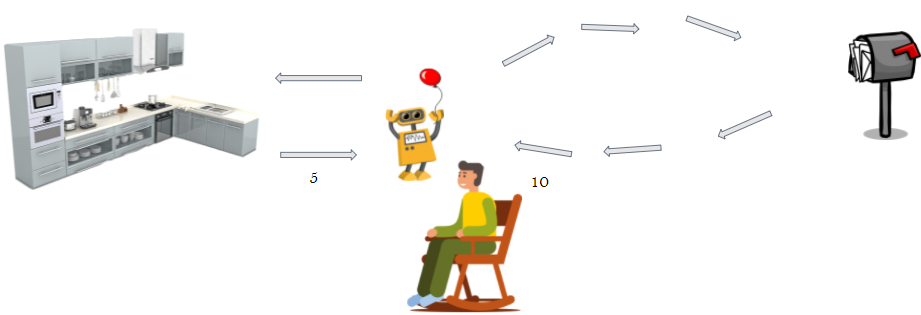
\includegraphics[width=10cm]{mot.png}
    %\caption{Caption}
    %\label{fig:my_label}
\end{figure}
\vfill\hfill\tiny{\href{https://www.emojipng.com/}{emojipng.com}}
\end{frame}

%------------------------------------------------

\begin{frame}
\frametitle{Average Reward Formulation}
\begin{block}{Objective}<1->
Maximize the expected average reward per stage:
    \[\rho^{\pi}(i)=\underset{N\rightarrow\infty}{\text{lim inf}}\dfrac{1}{N}E\Big\{\sum_{n=0}^{N-1}r(x_n,\mu_n(x_n))|x_0=i\Big\}\]
\end{block} 
\begin{block}{Definition}<1->
\begin{center}
$\pi^*$ is gain optimal if $\rho^{\pi^*}(s_0)\geq\rho^{\pi}(s_0)$ $\forall \pi$ and $\forall s_0 \in \mathcal{S}$\\
and hence $\pi^* \in \underset{\pi}{\text{arg max}} \rho^\pi$
\end{center}
\end{block} 

\end{frame}


    
%------------------------------------------------

\begin{frame}
\frametitle{Average Reward Formulation}
\begin{definition}
A Weak Accessibility (WA) condition holds if the set of states can be partitioned into two subsets $S_t$ and $S_c$ such that:\\
(i) All states in $S_t$ are transient under every stationary policy.\\
(ii) For every two states $i$ and $j$ in $S_c$, $j$ is accessible from $i$.
\end{definition}
\begin{definition}
\label{def:unichain}
An MDP is unichain if it consists of a single recurrent class and possibly some transient states.
\end{definition}
Under this condition:
\begin{block}{Important Result}<1->
\begin{center}
    $\rho^{\pi}(s) = \rho^{\pi}(s') = \rho^\pi$ $\forall \pi$ and $\forall s,s' \in \mathcal{S}$
\end{center}
\end{block}
\end{frame}

\begin{frame}
\frametitle{Average Reward Formulation}
\begin{block}{Definition}
We define bias value  $V_b^\pi(s_0)$ as the average adjusted sum of rewards from a policy

   \[ V_b^\pi(s_0) := \underset{N\rightarrow\infty}{\text{lim}} E\Big\{\sum_{n=0}^{N-1}\Big(r(x_n,\mu_n(x_n))-\rho^\pi\Big)|x_0=s_0\Big\}\]

where $\rho^\pi$ is the average reward associated with the policy $\pi$.\\
\end{block}
$V_b^\pi$ Bias value or Relative value
\[V_b^\pi(s)-V_b^\pi(s')\]
\end{frame}

%------------------------------------------------
\begin{frame}
\frametitle{Bellman Equation}
\begin{theorem}
For any unichain MDP, there exists a value function $V^*$ and a scalar $\rho^*$ satisfying the equation.
\[
    V^*(s)+\rho^* = \underset{a}{\text{max}}\Big\{r(s,a)+ \sum_{s'\in\mathcal{S}}p(s'|s,a)V^*(s')\Big\}  \hspace{10pt} \forall s \in \mathcal{S}\]

\end{theorem}
\end{frame}

%------------------------------------------------

\begin{frame}
\frametitle{Relative Value Iteration}
Consider the mapping
\[T(V)(s) = \underset{a}{\text{max}} \Big(r(s,a)+\sum_{s'}p(s'|s,a)V(s') \Big)\]

\begin{block}{RVI}
\begin{equation}
    V^{n+1}(s) = T(V^n)(s)-V^n(s_{\text{ref}})  \hspace{10pt}\forall s\in\mathcal{S}\nonumber
\end{equation}
where $s_{\text{ref}}$ is an arbitrary but fixed reference state. \\
\begin{center}
    \textit{It is shown that as} $n\rightarrow\infty$, $V^n(s_{\text{ref}})\rightarrow \rho^{\pi^*}$
\end{center}
\end{block}
\end{frame}

%------------------------------------------------
\begin{frame}{Relative Value Iteration}
Relative Value iteration with synchronous updates
    \[V^{n+1}(s) = \underset{a}{\text{max}}\Big\{r(s,a)+\sum_{s'}p(s'|s,a)V^n(s')\Big\} - V^n(s_{\text{ref}})\]
\end{frame}

%------------------------------------------------

\begin{frame}
\frametitle{RVI Q-Learning}
Now we define the the relative state action \textit{``Q-value''} as following\\
\[
    Q^{\pi}(s,a) := \underset{N\rightarrow\infty}{\text{lim}} E\Big\{\sum_{k=0}^{N-1}\Big(r(x_k,\mu_k(x_k))-\rho^\pi\Big)|x_0=s,u_0=a\Big\}\]
$\forall (s,a)\in \mathcal{S}\times\mathcal{A}$ 

\begin{block}{Bellman Optimality Equation for Q}
\[
    Q^*(s,a)+\rho^* = r(s,a)+\sum_{s'\in\mathcal{S}}p(s'|s,a)V_b^*(s') \hspace{10pt} \forall (s,a)\in \mathcal{S}\times\mathcal{A}\] 
where $V_b^*(s') = \underset{a'\in\mathcal{A}}{\text{max}}\ Q^*(s',a')$
\end{block}
\end{frame}


%------------------------------------------------

\begin{frame}
\frametitle{RVI Q-Learning}
\begin{block}{DP Equation}
\[Q^{n+1}(s,a) = r(s,a)+\sum_{s'\in\mathcal{S}}p(s'|s,a)\underset{a'\in\mathcal{A}}{\text{max}}\ Q^n(s',a')-\underset{a''\in\mathcal{A}}{\text{max}}\ Q^n(s_{\text{ref}},a'')\]
\end{block}

\begin{block}{RVI Q-learning}
\begin{eqnarray}
    Q^{n+1}(s,a) &=& Q^{n}(s,a) +a(n)\Big(r(s,a)+\underset{a'\in\mathcal{A}}{\text{max}}\ Q^n(\xi_{ia},a')\nonumber\\ 
    && -f(Q^n)-Q^{n}(s,a)\Big)\nonumber
\end{eqnarray}
\end{block}
\end{frame}

\begin{frame}{RVI Q-learning}
\begin{block}{Asynchronous RVI}
\begin{eqnarray}
    Q^{n+1}(i,u) &=& Q^{n}(i,u) +a(v(n,i,u))I\{X_n=i,U_n=u\}\Big(r(i,u)+\nonumber\\ &&\underset{v\in\mathcal{A}}{\text{max}}\ Q^n(X_{n+1},v)-f(Q^n)-Q^{n}(i,u)\Big)  \hspace{4cm} \forall (i,u)\in \mathcal{S}\times\mathcal{A}\nonumber
\end{eqnarray}
\end{block}

\begin{block}{Assumptions}
\begin{itemize}
    \item $f$ is Lipschitz and for $e$ equal to a constant vector of all 1's in $R^{d\times r}$, $f(e)=1$ and $f(x+ce)=f(x)+c$ for some scalar $c\in R$.
    \item Comparable exploration $\forall (i,u)\in \mathcal{S}\times\mathcal{A}$, mathematically $\exists $ $\Delta$ such that
\[\underset{n\rightarrow\infty}{\text{lim inf}}\ \dfrac{v(n,i,u)}{n+1}\geq \Delta \ \text{a.s}\]
\end{itemize}
\end{block}
\end{frame}
\begin{frame}
\Huge{\centerline{Break}}
\end{frame}

%------------------------------------------------
\begin{frame}{Classic DQN}
\begin{figure}
    \centering
    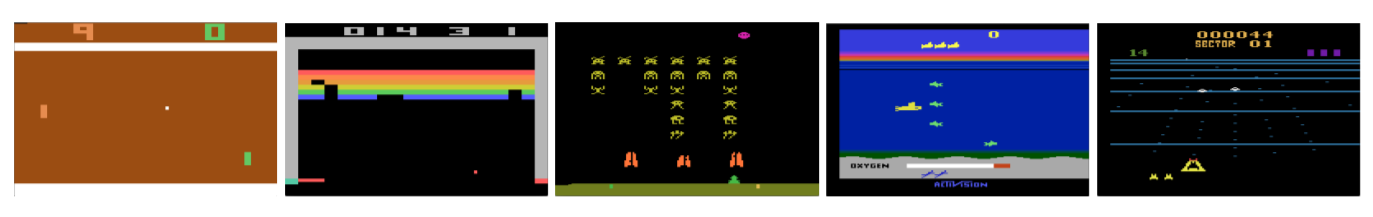
\includegraphics[width=7cm]{dqn.png}
    \caption{Atari Games}
    \label{fig:my_label}
\end{figure}
\begin{block}{True Bellman Error}
\begin{equation}
\bar{\mathcal{E}}(\theta) := E\Big[\Big(r(X_n, U_n) + \gamma\sum_{y\in\mathcal{S}} p(y|X_n,U_n)
\max_v Q(y,v; \theta) - Q(X_n,U_n;\theta)\ \Big)^2\Big] \label{Ebar}\nonumber
\end{equation}
\begin{center}
    $\gamma$ is discount factor
\end{center}
\end{block}
\end{frame}


\begin{frame}{DQN}
\begin{equation}
\theta_{n+1} = \theta_n +a(n)(Z_n - Q(X_n, U_n; \theta_n))\nabla_\theta Q(X_n, U_n; \theta_n), \quad n \geq 0 \nonumber \end{equation}

\begin{block}{Variants}
Vanilla DQN
\begin{equation}
Z_n := r(X_n,U_n)+\gamma \max_v Q(X_{n+1},v;\theta_n)\nonumber
\end{equation}
``Classic'' DQN
\begin{equation}
Z_n := r(X_n,U_n)+\gamma Q(X_{n+1},v;\theta_n')\Big|_{v = \mbox{argmax}_{v'} Q(X_{n+1}, v' ; \theta'_n)}\nonumber
\end{equation}
Double DQN
\begin{equation}
Z_n := r(X_n,U_n)+\gamma Q(X_{n+1},v;\theta_n')\Big|_{v = \mbox{argmax}_{v'} Q(X_{n+1}, v' ; \theta_n)}\nonumber
\end{equation}
\end{block}
\end{frame}

\begin{frame}{DQN}
    \begin{block}{Replay Buffer}
    We also maintain a replay buffer in we store the transitions $(X_n,U_n,R_n,X_{n+1})$. This leads to the term multiplying $a(n)$ in DQN iteration by an empirical average over past transitions.
\begin{eqnarray}
\theta_{n+1} &=& \theta_n + \frac{a(n)}{M}\times\sum_{m=1}^M\Bigg((Z_{n(m)}  - Q(X_{n(m)}, U_{n(m)}))\times\nonumber \\
&&\nabla_\theta Q(X_{n(m)}, U_{n(m)}; \theta_{n(m)})\Bigg), \ n \geq 0,\nonumber \label{DQN2}
\end{eqnarray}
where $(X_{n(m)}, U_{n(m)}),\ 1 \leq m \leq N,$ are samples from past. 
    \end{block}
\end{frame}

\begin{frame}{FGDQN}

\begin{block}{Full Gradient DQN}
\begin{eqnarray}
\theta_{n+1} &=& \theta_n - a(n)\left(r(X_n,U_n) + \gamma\max_v Q(X_{n+1}, v; \theta_n) - Q(X_n, U_n;\theta_n)\right)\times \nonumber \\
&& \left(\gamma\nabla_\theta Q(X_{n+1}, v_n; \theta_n) - \nabla_\theta Q(X_n, U_n; \theta_n)\right)\nonumber
\end{eqnarray}


\begin{eqnarray}
\theta_{n+1} &=& \theta_n - a(n)\Bigg(\overline{(r(X_n,U_n) + \gamma\max_v Q(X_{n+1}, v; \theta_n) - Q(X_n, U_n;\theta_n))}\times \nonumber \\
&& \left(\gamma\nabla_\theta Q(X_{n+1}, v_n; \theta_n) - \nabla_\theta Q(X_n, U_n; \theta_n)\right)  + \xi_{n+1}\Bigg)\nonumber
\end{eqnarray}
for $n \geq 0$, where $\{\xi_n\}$  is extraneous i.i.d.\  noise componentwise distributed independently and uniformly on $[-1,1]$
\end{block}

\end{frame}

\begin{frame}{Average Reward FGDQN}
    \begin{eqnarray}
    \bar{\mathcal{E}}(\theta) &=& E\Big[\Big(r(X_n, U_n) + \sum_{y\in\mathcal{S}} p(y|X_n,U_n)
\max_v Q(y,v; \theta) \nonumber \\&& -Q(X_n,U_n;\theta) - f(Q)\ \Big)^2\Big]\nonumber \label{Ebar}
    \end{eqnarray}
\begin{block}{Q iteration}
\begin{equation}
\theta_{n+1} = \theta_n +a(n)(Z_n - Q(X_n, U_n; \theta_n))\nabla_\theta Q(X_n, U_n; \theta_n), \quad n \geq 0 \nonumber
\end{equation}
\begin{eqnarray}
\label{eqn:fgdqnavg}
\theta_{n+1} &=& \theta_n - a(n)\Big(r(X_n,U_n) +\max_v Q(X_{n+1}, v; \theta_n) -f(Q;\theta_n) \nonumber \\
&&- Q(X_n, U_n;\theta_n)\Big)\times  \Big(\nabla_\theta Q(X_{n+1}, v_n; \theta_n) - \nabla_\theta f(Q;\theta_n) \nonumber \\
&&- \ \nabla_\theta Q(X_n, U_n; \theta_n)\Big)\nonumber \\
& \ \nonumber\label{Q-update0}
\end{eqnarray}

\end{block}

\end{frame}


\begin{frame}{Restless Bandits}
    Superscript $\alpha$ is used to indicate $\alpha$-th arm and $n, m$ are used to denote discrete time-steps.
\begin{itemize}
    \item Actions available are active $(u = 1)$ and passive $(u = 0)$.
    \item At each time $n$, we can activate exactly $M$ out of $N$ arms i.e. $\sum_{k=0}^N U_n^k = M \ \forall n$.
    \item Arms with action $u=0$ can possible evolve and accrue reward in a distinct way when $u=1$. 
\end{itemize}
\begin{block}{Objective}
The objective is to maximize long run average reward 
\begin{equation}
\label{eqn:wobj}
\liminf_{n\rightarrow\infty}\frac{1}{n}E\left[\sum_{m=0}^{n-1}\sum_{\alpha=1}^Nr^\alpha(X^\alpha_m, U^\alpha_m)\right]\nonumber
\end{equation}
\end{block}

\end{frame}


\begin{frame}{Whittle's Approach}
    \begin{block}{Simplification of the constraint}
    \begin{equation}
\liminf_{n\rightarrow\infty}\frac{1}{n}E\left[\sum_{m=0}^{n-1}\sum_{\alpha=1}^NU^\alpha_m\right] = M \label{constraint2}\nonumber
\end{equation}
\begin{center}
    `per time instant' $\rightarrow$ `time-averaged constraint'
\end{center}

    \end{block}
\begin{block}{Lagrangian Relaxation}
\begin{equation}
\liminf_{n\rightarrow\infty}\frac{1}{n}E\left[\sum_{m=0}^{n-1}\sum_{\alpha=1}^N\Big(r^\alpha(X^\alpha_m, U^\alpha_m)+\lambda(1-U_m^\alpha)\Big)\right]+\lambda M \label{reward}\nonumber
\end{equation}
\begin{center}
    $\lambda \rightarrow$ Lagrange Multiplier\\
    `subsidy for passive action' 
\end{center}
\end{block}
\end{frame}

\begin{frame}{Whittle Index}
    \begin{block}{Indexability Criteria}
    An arm $\alpha$ is considered to be \textit{indexable} if the set $\mathcal{P}$ increases monotonically from $\Phi$ to the entire state space as we increase $\lambda^\alpha$ (the subsidy for passive action). The RMAB problem is \textit{indexable} if all $N$ arms are \textit{indexable}.
    \end{block}
\begin{figure}
    \centering
    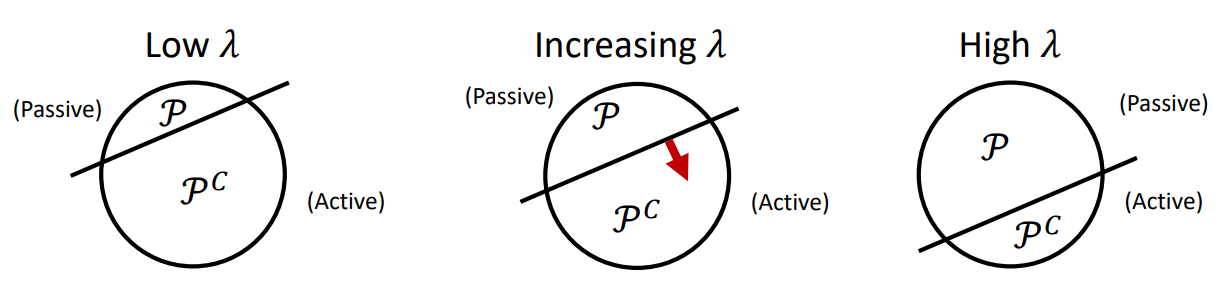
\includegraphics[width=8cm]{whittle1.png}
    \caption{Indexability}
    \label{fig:my_label}
\end{figure}
$\mathcal{P}$ and $\mathcal{P}^C$ denote set of state-space for which $u = 0, u = 1$ are optimal actions resp.

\end{frame}

\begin{frame}{Whittle Index}
    \begin{block}{Whittle Index}
    For an arm $\alpha$, Whittle index is defined as the $\lambda^\alpha = \text{inf}\ \{\lambda^\alpha: \alpha \in \mathcal{P}\}$. It is the infimum subsidy $\lambda^\alpha$ one has to pay so that it is equally desirable to give an arm $\alpha$ active action and passive action.
    \end{block}
\begin{figure}
    \centering
    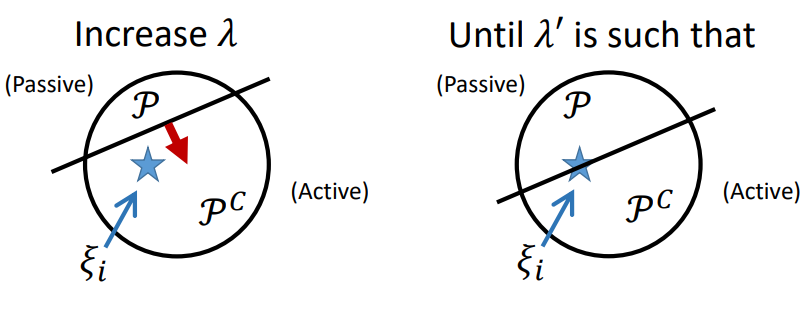
\includegraphics[width=5cm]{whittle2.png}
    \caption{$\lambda'$ is whittle index}
    \label{fig:my_label}
\end{figure}   
\begin{block}{Whittle Index Policy}
Policy which activates or gives active actions to those $M$ arms out of $N$ which has highest whittle indices $\lambda$.  
\end{block}
\end{frame}


\begin{frame}{Q-learning for Whittle Index}
\begin{block}{Dynamic Programming equation}
\begin{eqnarray}
Q(i,u) &=& ur(i,1) + (1-u)(\lambda + r(i,0)) - \rho\nonumber \\
&& + \sum_j p(j|i,u)\max_v Q(j,v)\nonumber \label{Q-DP}
\end{eqnarray}
\end{block}
\begin{block}{Whittle Index Definition}
\begin{eqnarray}
\lambda(\hat{k}) := r(\hat{k},1) + \sum_jp(j | \hat{k}, 1)V(j)
- r(\hat{k},0) - \sum_jp(j | \hat{k}, 0)V(j)\nonumber \label{Windex0}
\end{eqnarray}
This is equivalent to solving
\begin{equation}
Q(\hat{k}, 1) - Q(\hat{k}, 0)=0\nonumber \label{Windex}
\end{equation}
for $\lambda = \lambda(\hat{k})$
\end{block}
\end{frame}

\begin{frame}{Q-learning for Whittle Index}
\begin{block}{Two Time Scale Algorithm}
We update $Q-$values on a faster time scale and $\lambda$ on a slower time scale.
\begin{eqnarray}
Q_{n+1}(i,u;\hat{k}) &=& Q_n(i,u;\hat{k})  +   a(\nu(i,u,n))I\{X_n = i, U_n = u\} \nonumber \\
&& \times \Big((1 - u)(r(i,0) + \lambda_n(\hat{k})) + ur(i,1) +  \nonumber \\
&& \max_{v\in\U}Q_n(X_{n+1},v;\hat{k})  - f(Q_n(\hat{k})) - Q_n(i,u;\hat{k})\Big)\nonumber
\end{eqnarray}
\begin{equation}
\lambda_{n+1}(\hat{k}) = \lambda_n(\hat{k}) + b(n) \left( Q_n(\hat{k},1;\hat{k}) - Q_n(\hat{k},0;\hat{k}) \right)\nonumber
\label{lambda-update}
\end{equation}
where stepsize sequence $\{b(n)\}$ satisfies $b(n) = o(a(n))$.
\end{block}
\end{frame}

\begin{frame}{FGDQN for Whittle Index}
\begin{block}{Proof}
\begin{equation}
    Q(\hat{k}_n,1) = Q(\hat{k}_n,0)\nonumber
\end{equation}
\begin{equation}
    \lambda(\hat{k}_n) = Q(\hat{k}_n,1)-r(\hat{k}_n,0)+\rho-\sum p(\hat{k}_{n+1}|\hat{k}_n,0)\max_{v\in\{0,1\}}Q(\hat{k}_{n+1},v;\theta_n)\nonumber
\end{equation} 
We consider a single run $\{X_n=\hat{k}_n,U_n=0\}$ of the controlled Markov chain which gives $\hat{k}_{n+1}$ with the law $p(\cdot|\hat{k}_n,0)$. 
\\Using stochastic approximation we remove the conditional expectation by a real random variable and make increment based on our current estimate.
\\$\therefore$ We now know have,
\begin{eqnarray}
\lambda(X_n) &=& (1-b(n))\lambda(X_n)+ I\{X_n=\hat{k}_n,U_n=0\}b(n)\Big(Q(X_n,1)\nonumber \\
&&-r(X_n,0)+\rho-\max_{v\in\{0,1\}}Q(X_{n+1},v;\theta_n)\Big)\nonumber
\end{eqnarray}

\end{block}
\end{frame}




\begin{frame}{FGDQN for Whittle Index}
\begin{block}{Modified $\lambda$ iteration}
\begin{eqnarray}
\label{whittleiteration}
\lambda(X_n) &=& \lambda(X_n)+ I\{X_n=\hat{k}_n,U_n=0\}b(\mu(i,0,n)) \Big(Q(X_n,1)-r(X_n,0)\nonumber \\&&+f(Q_n)-\max_{v\in\{0,1\}}Q(X_{n+1},v;\theta_n)-\lambda(X_n))\Big)\nonumber
\end{eqnarray}
here, $\mu(i,0,n)$ is a local clock for Whittle Index and $b=o(a(n))$.\\
Following we get the iteration for Whittle Index parameters $\theta'$

\begin{eqnarray}
\theta'_{n+1} &=& \theta'_n+b(n)I\{U_n=0\}\times\Big(Q(X_n,1;\theta_n)-r(X_n,0)+f(Q_n)\nonumber \\&&
-\max_{v\in\{0,1\}} Q(X_{n+1}, v; \theta_n)-\lambda(X_n;\theta'_n)\Big)\nabla_{\theta'}\lambda(X_n;\theta'_n)\nonumber
\label{method2}\end{eqnarray}
\end{block}
    
\end{frame}

\begin{frame}{Experiments}
Whittle Index
\begin{figure}[H]
     \captionsetup[subfigure]{justification=centering}
     \centering
     %\hspace{-0.26\linewidth}
     \begin{subfigure}{0.4\linewidth}
         \centering
         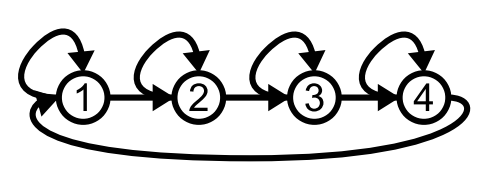
\includegraphics[width=0.7\linewidth]{circac.png}
         \caption{Action Action}
         \label{}
     \end{subfigure}
     \begin{subfigure}{0.4\linewidth}
         \centering
         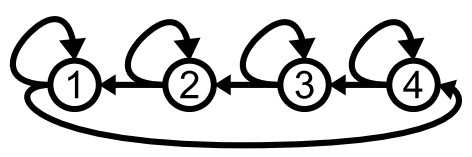
\includegraphics[width=0.7\linewidth]{circpas.png}
         \caption{Passive Action}
         \label{}
     \end{subfigure}
     %\hspace{0.2\linewidth}
     %\hspace{0.2\linewidth}
     \caption{Underlying Markov chains of the Circulant Dynamics Problem}
     \label{Circulant Dynamics}
\end{figure}
Transition probability matrix $P_0=\left[\begin{array}{cccc}
{\small 1/2} & 0 & 0 & 1/2\\
1/2 & 1/2 & 0 & 0\\
0 & 1/2 & 1/2 & 0\\
0 & 0 & 1/2 & 1/2
\end{array}\right], \quad \mbox{and} \quad
P_1=P_0^T,$ for passive and active action respectively. \\The rewards here do not depend on action and are given by $R(1,0)=R(1,1)=-1$, $R(2,0)=R(2,1)=0$, $R(3,0)=R(3,1)=0$, and $R(4,0)=R(4,1)=1$.
\end{frame}
\begin{frame}{Experiments - Whittle Index 1}
    \begin{figure}[H]
\ContinuedFloat
     \captionsetup[subfigure]{justification=centering}
     \centering
     %\hspace{-0.26\linewidth}
     \begin{subfigure}{0.48\linewidth}
         \centering
         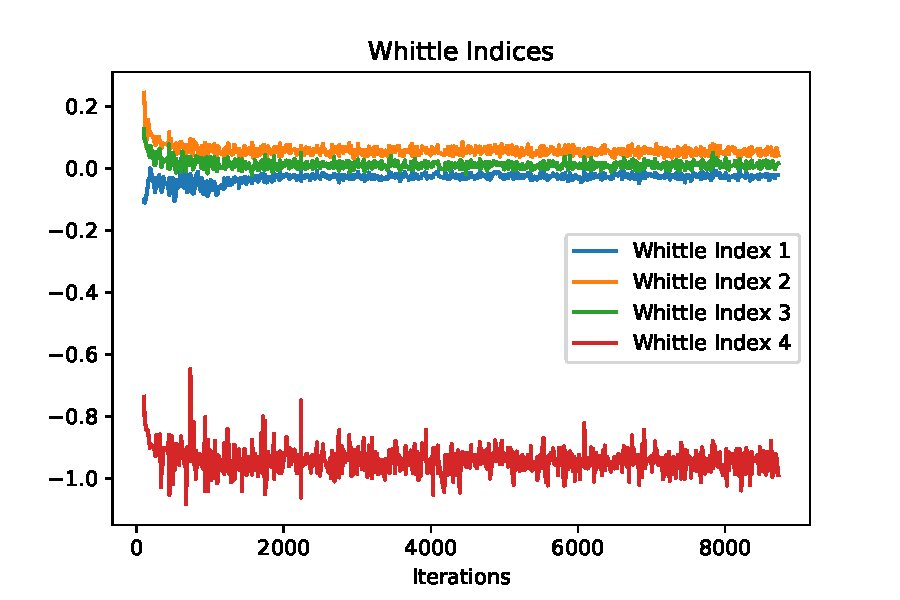
\includegraphics[width=0.8\linewidth]{all.pdf}
         \caption{Whittle Indices}
         \label{Whittle Indices1}
     \end{subfigure}
     \begin{subfigure}{0.48\linewidth}
         \centering
         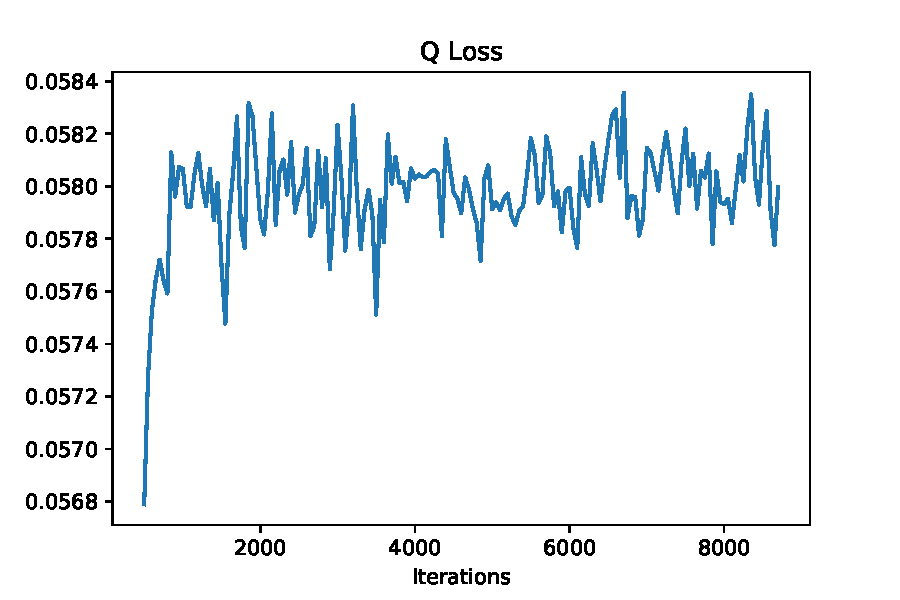
\includegraphics[width=0.8\linewidth]{Q Loss.pdf}
         \caption{Q loss}
         \label{}
     \end{subfigure}
     
     \begin{subfigure}{0.48\linewidth}
         \centering
         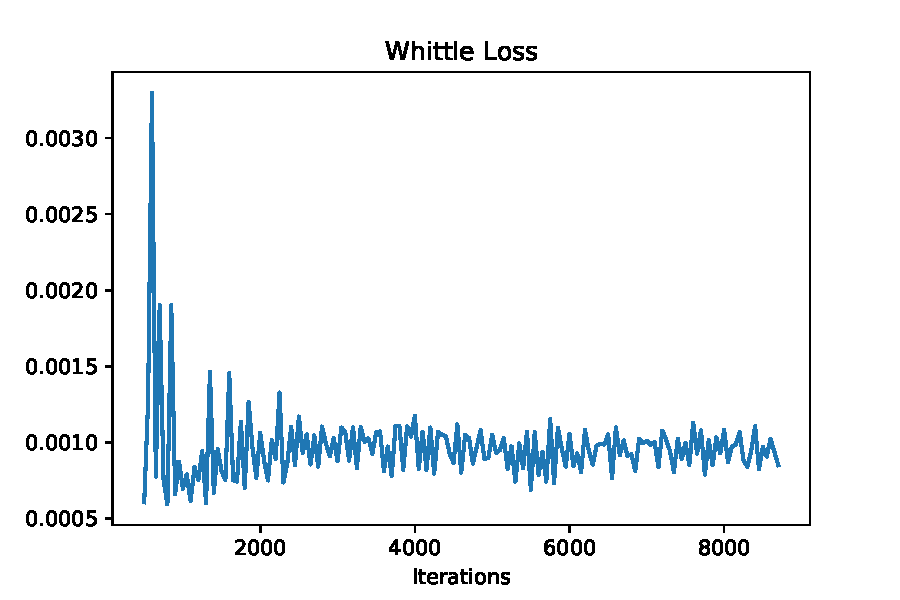
\includegraphics[width=0.8\linewidth]{Whittle Loss.pdf}
         \caption{Whittle loss}
         \label{}
     \end{subfigure}
     %\hspace{0.2\linewidth}
     %\hspace{0.2\linewidth}
     \caption{Circulant Dynamics}
     \label{}
\end{figure}

\end{frame}
\begin{frame}{Experiments - Whittle Index 2}
    The active action forces an arm to restart from some state. 
    Consider an example with 5 states, where in the passive mode ($u=0$) an arm has tendency to go up the state space, and in the active mode ($u=1$) the arm restarts from state 1 with probability 1
$$
P_0=\left[\begin{array}{ccccc}
1/10 & 9/10 & 0 & 0 & 0\\
1/10 & 0 & 9/10 & 0 & 0\\
1/10 & 0 & 0 & 9/10 & 0\\
1/10 & 0 & 0 & 0 & 9/10\\
1/10 & 0 & 0 & 0 & 9/10
\end{array}\right], \quad P_1=\left[\begin{array}{ccccc}
1 & 0 & 0 & 0 & 0\\
1 & 0 & 0 & 0 & 0\\
1 & 0 & 0 & 0 & 0\\
1 & 0 & 0 & 0 & 0\\
1 & 0 & 0 & 0 & 0
\end{array}\right].
$$

% $$
% P_1=\left[\begin{array}{ccccc}
% 1 & 0 & 0 & 0 & 0\\
% 1 & 0 & 0 & 0 & 0\\
% 1 & 0 & 0 & 0 & 0\\
% 1 & 0 & 0 & 0 & 0\\
% 1 & 0 & 0 & 0 & 0
% \end{array}\right].
% $$
The rewards in the passive mode are given by $R(k,0)=\alpha^k$ ($\alpha$ is taken to be 0.9) and the rewards in the active mode are all zero.\\
\end{frame}

\begin{frame}{Experiments - Whittle Index 2}
    \begin{figure}[H]
     \captionsetup[subfigure]{justification=centering}
     \centering
     %\hspace{-0.26\linewidth}
     \begin{subfigure}{0.48\linewidth}
         \centering
         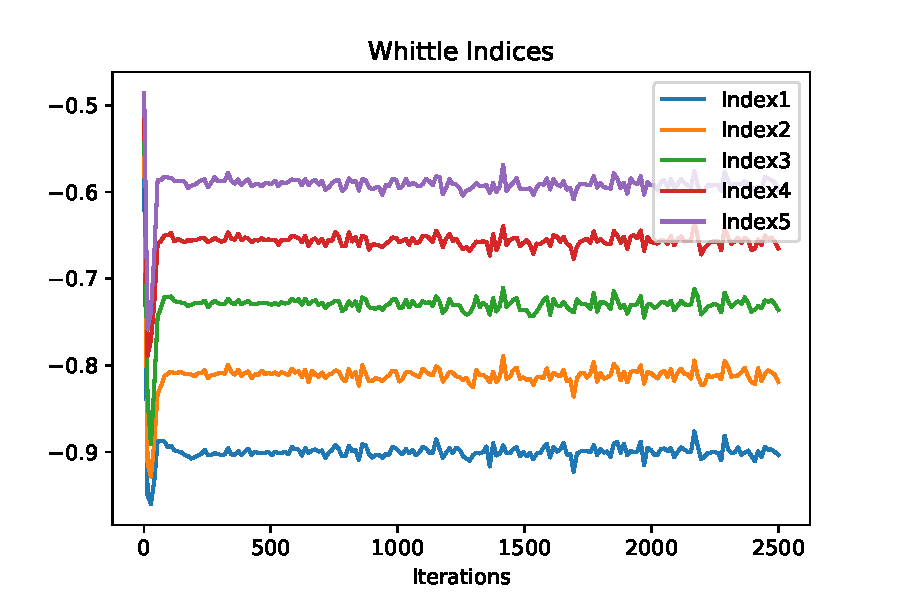
\includegraphics[width=1\linewidth]{Indices.pdf}
         \caption{Whittle Indices}
         \label{Whittle Indices 2}
     \end{subfigure}
     \begin{subfigure}{0.48\linewidth}
         \centering
         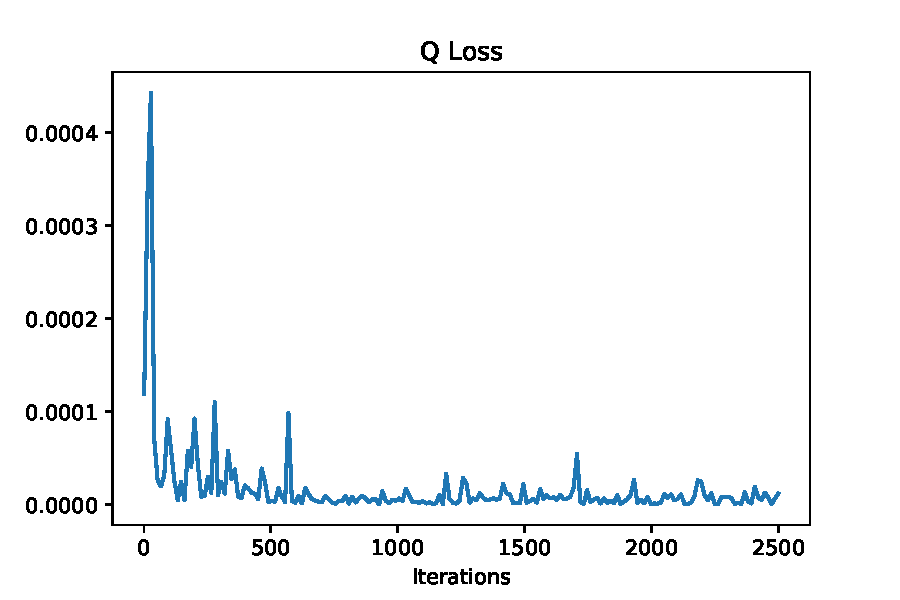
\includegraphics[width=1\linewidth]{Q Loss1.pdf}
         \caption{Q loss}
         \label{}
     \end{subfigure}
     %\hspace{0.2\linewidth}
     %\hspace{0.2\linewidth}
     \caption{Circulant Dynamics with Restart}
\end{figure}
\end{frame}
\begin{frame}
\Huge{\centerline{The End}}
\end{frame}

%----------------------------------------------------------------------------------------
\end{document} 